% Figures of doc/WZIP_format.md; one page each (build.sh turns page k into the SVG named in figures.txt)
\documentclass[tikz,border=8pt]{standalone}
\usepackage{xcolor}
\pagecolor{white}
\usetikzlibrary{positioning,decorations.pathreplacing,calc,arrows.meta,matrix}
% colors and styles shared by the figures of doc/
\definecolor{hdr}{HTML}{FFF2B3}   % size and other headers
\definecolor{tok}{HTML}{C9DCF5}   % tokens, joint symbols
\definecolor{lit}{gray}{0.86}      % literals
\definecolor{off}{HTML}{FAD7B5}   % offset fields
\definecolor{ext}{HTML}{CDEBC7}   % extensions and extra bits
\definecolor{flg}{HTML}{F2A65A}   % flags
\definecolor{endm}{HTML}{F5C2C2}  % end markers
\definecolor{tab}{HTML}{E3D5F2}   % code tables
\definecolor{b1}{HTML}{FBE3CC}    % one, two, three offset bytes
\definecolor{b2}{HTML}{F5BE8A}
\definecolor{b3}{HTML}{E8914A}
\tikzset{
  fld/.style={draw, minimum height=9mm, inner sep=2pt, align=center},
  brc/.style={decorate, decoration={brace, amplitude=4pt}},
  mbrc/.style={decorate, decoration={brace, mirror, amplitude=4pt}}}

\begin{document}

%% 1. wzip-stream: the one-call stream, a WZIP_L payload, a sequence block
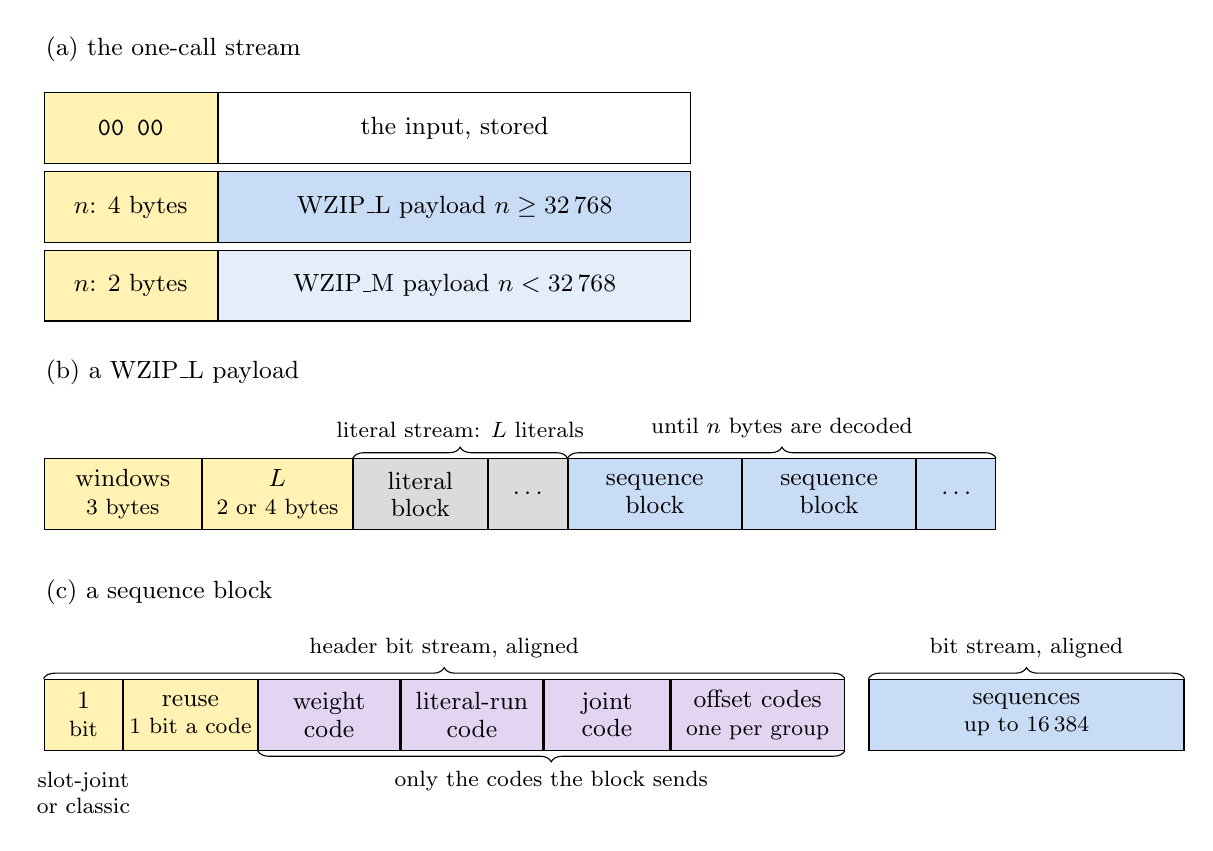
\begin{tikzpicture}[font=\small, node distance=0pt]
\node[anchor=west] at (-0.1,1.0) {(a) the one-call stream};
\node[fld, fill=hdr, minimum width=22mm] (a1) at (1.1,0) {\texttt{00 00}};
\node[fld, minimum width=60mm, right=of a1] {the input, stored};
\node[fld, fill=hdr, minimum width=22mm] (b1) at (1.1,-1.0) {$n$: 4 bytes};
\node[fld, fill=tok, minimum width=60mm, right=of b1] {WZIP\_L payload \hfill $n\ge 32\,768$};
\node[fld, fill=hdr, minimum width=22mm] (c1) at (1.1,-2.0) {$n$: 2 bytes};
\node[fld, fill=tok!50, minimum width=60mm, right=of c1] {WZIP\_M payload \hfill $n<32\,768$};
\node[anchor=west] at (-0.1,-3.1) {(b) a WZIP\_L payload};
\node[fld, fill=hdr, minimum width=20mm, align=center] (w) at (1.0,-4.65) {windows\\[-1pt]\footnotesize 3 bytes};
\node[fld, fill=hdr, minimum width=19mm, right=of w, align=center] (lc) {$L$\\[-1pt]\footnotesize 2 or 4 bytes};
\node[fld, fill=lit, minimum width=17mm, right=of lc, align=center] (lb1) {literal\\[-1pt]block};
\node[fld, fill=lit, minimum width=10mm, right=of lb1] (lb2) {$\cdots$};
\node[fld, fill=tok, minimum width=22mm, right=of lb2, align=center] (sb1) {sequence\\[-1pt]block};
\node[fld, fill=tok, minimum width=22mm, right=of sb1, align=center] (sb2) {sequence\\[-1pt]block};
\node[fld, fill=tok, minimum width=10mm, right=of sb2] (sb3) {$\cdots$};
\draw[brc] (lb1.north west) -- (lb2.north east) node[midway, above=4pt, font=\footnotesize] {literal stream: $L$ literals};
\draw[brc] (sb1.north west) -- (sb3.north east) node[midway, above=4pt, font=\footnotesize] {until $n$ bytes are decoded};
\node[anchor=west] at (-0.1,-5.9) {(c) a sequence block};
\node[fld, fill=hdr, minimum width=10mm, align=center] (sj) at (0.5,-7.45) {1\\[-1pt]\footnotesize bit};
\node[fld, fill=hdr, minimum width=14mm, right=of sj, align=center] (ru) {reuse\\[-1pt]\footnotesize 1 bit a code};
\node[fld, fill=tab, minimum width=18mm, right=of ru, align=center] (wc) {weight\\[-1pt]code};
\node[fld, fill=tab, minimum width=18mm, right=of wc, align=center] (t1) {literal-run\\[-1pt]code};
\node[fld, fill=tab, minimum width=16mm, right=of t1, align=center] (t2) {joint\\[-1pt]code};
\node[fld, fill=tab, minimum width=22mm, right=of t2, align=center] (t3) {offset codes\\[-1pt]\footnotesize one per group};
\node[fld, fill=tok, minimum width=40mm, right=3mm of t3, align=center] (sq) {sequences\\[-1pt]\footnotesize up to 16\,384};
\draw[brc] (sj.north west) -- (t3.north east) node[midway, above=4pt, font=\footnotesize] {header bit stream, aligned};
\draw[mbrc] (wc.south west) -- (t3.south east) node[midway, below=4pt, font=\footnotesize] {only the codes the block sends};
\draw[brc] (sq.north west) -- (sq.north east) node[midway, above=4pt, font=\footnotesize] {bit stream, aligned};
\node[below=1.5mm of sj, font=\footnotesize, align=center] {slot-joint\\or classic};
\end{tikzpicture}

%% 2. wzip-parse: a parse, its literal stream and its sequences
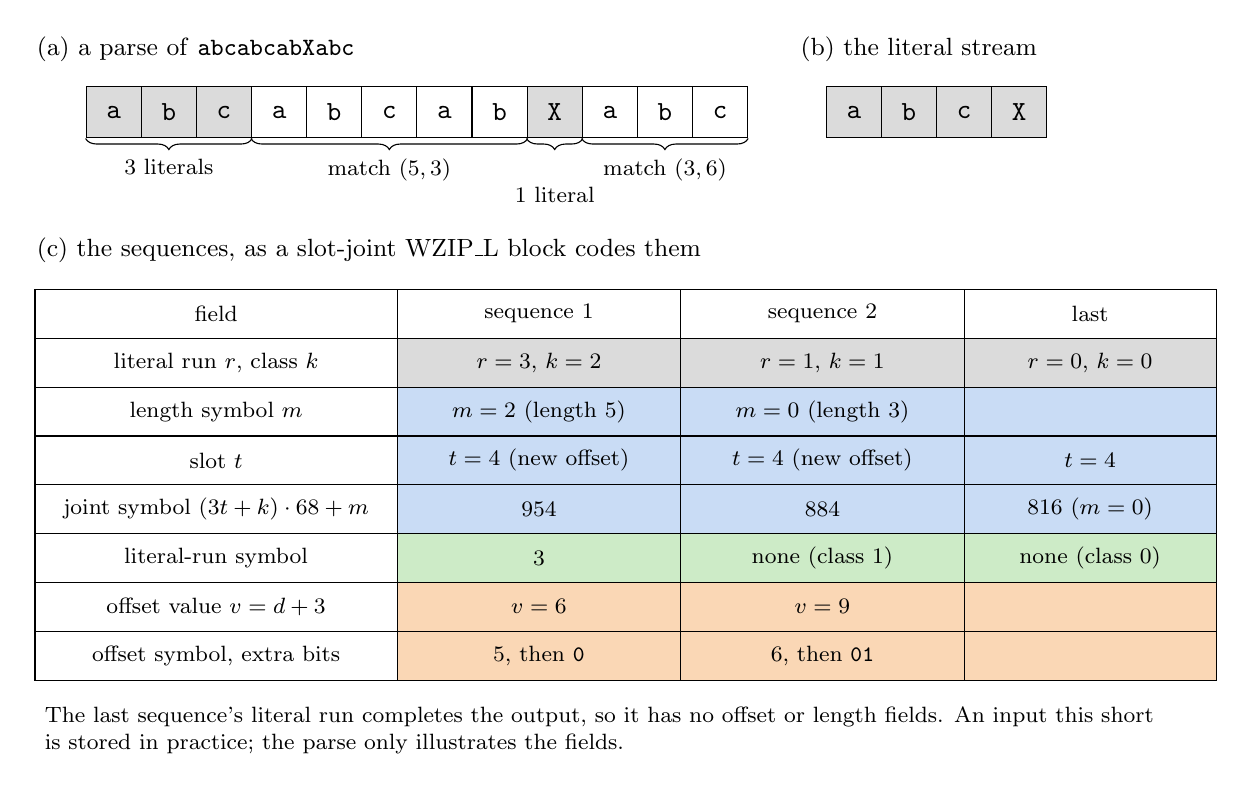
\begin{tikzpicture}[font=\small,
  cell/.style={draw, minimum width=7mm, minimum height=6.5mm, inner sep=0pt, font=\ttfamily},
  tcell/.style={draw, minimum height=6.5mm, inner sep=2pt, font=\footnotesize, align=center}]
\node[anchor=west] at (-0.4,0.8) {(a) a parse of \texttt{abcabcabXabc}};
\foreach \c/\f [count=\i] in {a/lit,b/lit,c/lit,a/white,b/white,c/white,a/white,b/white,X/lit,a/white,b/white,c/white}
  \node[cell, fill=\f] (x\i) at (0.7*\i,0) {\c};
\draw[mbrc] (x1.south west) -- (x3.south east) node[midway, below=4pt, font=\footnotesize] {3 literals};
\draw[mbrc] (x4.south west) -- (x8.south east) node[midway, below=4pt, font=\footnotesize] {match $(5,3)$};
\draw[mbrc] (x9.south west) -- (x9.south east) node[midway, below=14pt, font=\footnotesize] {1 literal};
\draw[mbrc] (x10.south west) -- (x12.south east) node[midway, below=4pt, font=\footnotesize] {match $(3,6)$};
\node[anchor=west] at (9.3,0.8) {(b) the literal stream};
\foreach \c [count=\i] in {a,b,c,X} \node[cell, fill=lit] at (9.4+0.7*\i,0) {\c};
\node[anchor=west] at (-0.4,-1.75) {(c) the sequences, as a slot-joint WZIP\_L block codes them};
\newcommand{\trow}[6]{% row, fill, four cells
  \foreach \xa/\xb/\t [count=\c] in {-0.3/4.3/{#3}, 4.3/7.9/{#4}, 7.9/11.5/{#5}, 11.5/14.7/{#6}} {
    \ifnum\c=1 \draw (\xa,-2.25-0.62*#1) rectangle (\xb,-2.87-0.62*#1);
    \else \draw[fill=#2] (\xa,-2.25-0.62*#1) rectangle (\xb,-2.87-0.62*#1); \fi
    \node[font=\footnotesize] at ({(\xa+\xb)/2},-2.56-0.62*#1) {\t};}}
\trow{0}{white}{field}{sequence 1}{sequence 2}{last}
\trow{1}{lit}{literal run $r$, class $k$}{$r=3$, $k=2$}{$r=1$, $k=1$}{$r=0$, $k=0$}
\trow{2}{tok}{length symbol $m$}{$m=2$ (length 5)}{$m=0$ (length 3)}{}
\trow{3}{tok}{slot $t$}{$t=4$ (new offset)}{$t=4$ (new offset)}{$t=4$}
\trow{4}{tok}{joint symbol $(3t+k)\cdot 68+m$}{954}{884}{816 ($m=0$)}
\trow{5}{ext}{literal-run symbol}{3}{none (class 1)}{none (class 0)}
\trow{6}{off}{offset value $v=d+3$}{$v=6$}{$v=9$}{}
\trow{7}{off}{offset symbol, extra bits}{5, then \texttt{0}}{6, then \texttt{01}}{}
\node[anchor=west, font=\footnotesize, align=left] at (-0.3,-7.85) {The last sequence's literal run completes the output, so it has no offset or length fields. An input this short\\is stored in practice; the parse only illustrates the fields.};
\end{tikzpicture}

%% 3. wzip-windows: the window schedule of a 16 MiB input, and its header
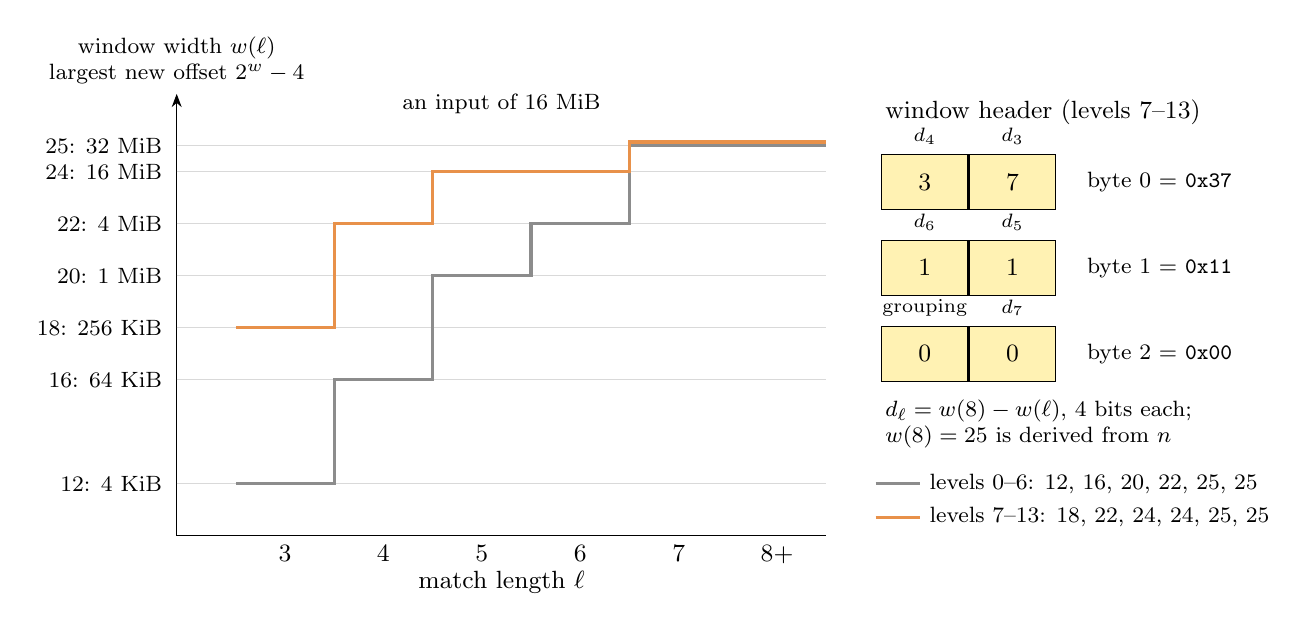
\begin{tikzpicture}[font=\small, x=1.25cm, y=0.33cm]
\draw[-{Stealth}] (2.4,10) -- (2.4,27) node[above, align=center, font=\footnotesize] {window width $w(\ell)$\\largest new offset $2^{w}-4$};
\draw (2.4,10) -- (9.0,10);
\foreach \y/\t in {12/{12: 4 KiB}, 16/{16: 64 KiB}, 18/{18: 256 KiB}, 20/{20: 1 MiB}, 22/{22: 4 MiB}, 24/{24: 16 MiB}, 25/{25: 32 MiB}} {
  \draw[black!15] (2.4,\y) -- (9.0,\y);
  \node[anchor=east, font=\footnotesize] at (2.35,\y) {\t};}
\foreach \x/\t in {3/3, 4/4, 5/5, 6/6, 7/7, 8/{8+}} \node[below, font=\small] at (\x+0.5,10) {\t};
\node[font=\small] at (5.7,8.2) {match length $\ell$};
% base schedule (levels 0-6) and the optimal levels' (7-13)
\draw[very thick, black!45] (3,12) -- (4,12) -- (4,16) -- (5,16) -- (5,20) -- (6,20) -- (6,22) -- (7,22) -- (7,25) -- (9,25);
\draw[very thick, b3] (3,18) -- (4,18) -- (4,22) -- (5,22) -- (5,24) -- (7,24) -- (7,25.15) -- (9,25.15);
\draw[very thick, black!45] (9.5,12.0) -- (9.95,12.0);
\node[anchor=west, font=\footnotesize] at (9.95,12.0) {levels 0--6: 12, 16, 20, 22, 25, 25};
\draw[very thick, b3] (9.5,10.7) -- (9.95,10.7);
\node[anchor=west, font=\footnotesize] at (9.95,10.7) {levels 7--13: 18, 22, 24, 24, 25, 25};
% the header of the optimal levels' schedule
\node[anchor=west] at (9.5,26.3) {window header (levels 7--13)};
\foreach \hi/\lo/\hl/\ll/\byte [count=\i from 0] in {3/7/{$d_4$}/{$d_3$}/37, 1/1/{$d_6$}/{$d_5$}/11, 0/0/{grouping}/{$d_7$}/00} {
  \node[draw, fill=hdr, minimum width=11mm, minimum height=7mm] (hi\i) at (10.0,23.6-3.3*\i) {\hi};
  \node[draw, fill=hdr, minimum width=11mm, minimum height=7mm, right=0pt of hi\i] (lo\i) {\lo};
  \node[font=\scriptsize, above=0pt of hi\i] {\hl};
  \node[font=\scriptsize, above=0pt of lo\i] {\ll};
  \node[anchor=west, font=\footnotesize] at (11.55,23.6-3.3*\i) {byte \i\ = \texttt{0x\byte}};}
\node[anchor=west, font=\footnotesize, align=left] at (9.5,14.3) {$d_\ell = w(8) - w(\ell)$, 4 bits each;\\$w(8)=25$ is derived from $n$};
\node[font=\footnotesize] at (5.7,26.6) {an input of 16 MiB};
\end{tikzpicture}

%% 4. wzip-sequence: the fields of a WZIP_L sequence and the joint alphabet
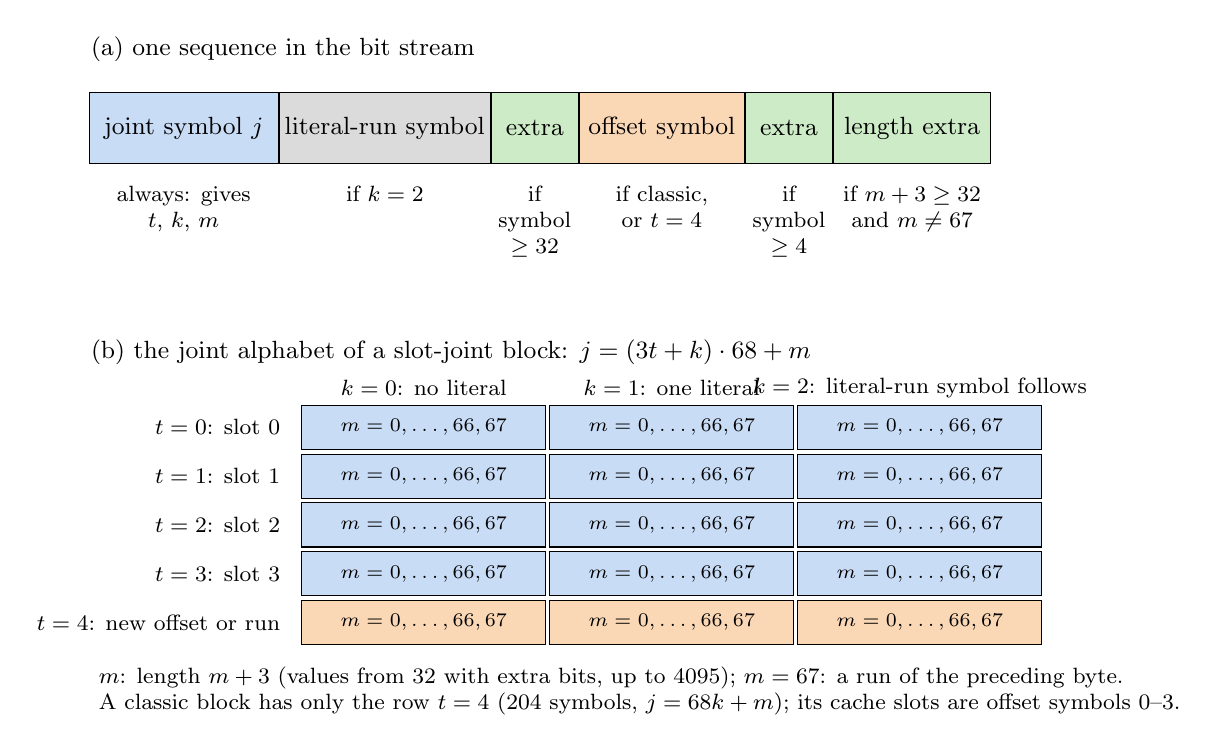
\begin{tikzpicture}[font=\small, node distance=0pt]
\node[anchor=west] at (-0.1,1.0) {(a) one sequence in the bit stream};
\node[fld, fill=tok, minimum width=24mm] (j) at (1.2,0) {joint symbol $j$};
\node[fld, fill=lit, minimum width=26mm, right=of j] (lr) {literal-run symbol};
\node[fld, fill=ext, minimum width=11mm, right=of lr] (lre) {extra};
\node[fld, fill=off, minimum width=21mm, right=of lre] (os) {offset symbol};
\node[fld, fill=ext, minimum width=11mm, right=of os] (ose) {extra};
\node[fld, fill=ext, minimum width=20mm, right=of ose] (le) {length extra};
\node[below=1.5mm of j, font=\footnotesize, align=center] {always: gives\\$t$, $k$, $m$};
\node[below=1.5mm of lr, font=\footnotesize, align=center] {if $k=2$};
\node[below=1.5mm of lre, font=\footnotesize, align=center] {if\\symbol\\$\ge 32$};
\node[below=1.5mm of os, font=\footnotesize, align=center] {if classic,\\or $t=4$};
\node[below=1.5mm of ose, font=\footnotesize, align=center] {if\\symbol\\$\ge 4$};
\node[below=1.5mm of le, font=\footnotesize, align=center] {if $m+3\ge 32$\\and $m\ne 67$};
\node[anchor=west] at (-0.1,-2.85) {(b) the joint alphabet of a slot-joint block: $j = (3t+k)\cdot 68 + m$};
\foreach \t/\tl/\f in {0/{slot 0}/tok, 1/{slot 1}/tok, 2/{slot 2}/tok, 3/{slot 3}/tok, 4/{new offset or run}/off} {
  \node[anchor=east, font=\footnotesize] at (2.55,-3.8-0.62*\t) {$t=\t$: \tl};
  \foreach \k in {0,1,2} {
    \node[draw, fill=\f, minimum width=31mm, minimum height=5.6mm, font=\scriptsize]
      at (4.25+3.15*\k,-3.8-0.62*\t) {$m = 0, \ldots, 66, 67$};}}
\foreach \k/\kl in {0/{$k=0$: no literal}, 1/{$k=1$: one literal}, 2/{$k=2$: literal-run symbol follows}}
  \node[font=\footnotesize] at (4.25+3.15*\k,-3.3) {\kl};
\node[anchor=west, font=\footnotesize, align=left] at (0,-7.15) {$m$: length $m+3$ (values from 32 with extra bits, up to 4095); $m=67$: a run of the preceding byte.\\A classic block has only the row $t=4$ (204 symbols, $j=68k+m$); its cache slots are offset symbols 0--3.};
\end{tikzpicture}

%% 5. wzip-literals: the literal stream's blocks
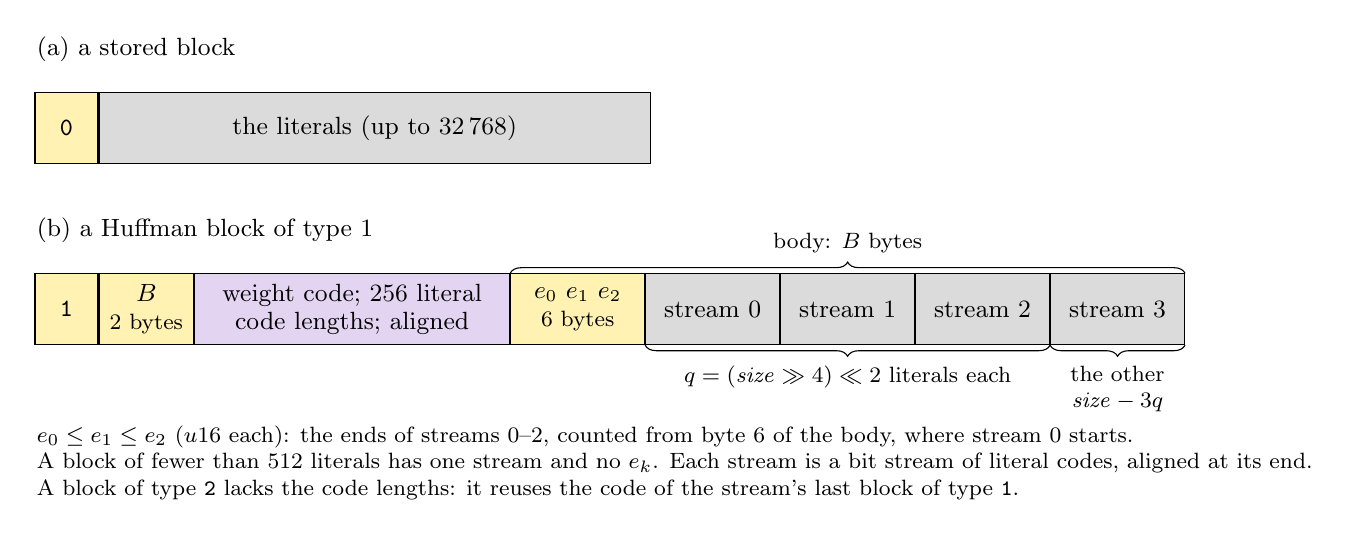
\begin{tikzpicture}[font=\small, node distance=0pt]
\node[anchor=west] at (-0.1,1.0) {(a) a stored block};
\node[fld, fill=hdr, minimum width=8mm] (s0) at (0.4,0) {\texttt{0}};
\node[fld, fill=lit, minimum width=70mm, right=of s0] {the literals (up to 32\,768)};
\node[anchor=west] at (-0.1,-1.3) {(b) a Huffman block of type 1};
\node[fld, fill=hdr, minimum width=8mm] (h0) at (0.4,-2.3) {\texttt{1}};
\node[fld, fill=hdr, minimum width=12mm, right=of h0, align=center] (hb) {$B$\\[-1pt]\footnotesize 2 bytes};
\node[fld, fill=tab, minimum width=40mm, right=of hb, align=center] (hc) {weight code; 256 literal\\[-1pt]code lengths; aligned};
\node[fld, fill=hdr, minimum width=17mm, right=of hc, align=center] (he) {$e_0$ $e_1$ $e_2$\\[-1pt]\footnotesize 6 bytes};
\node[fld, fill=lit, minimum width=17mm, right=of he] (q0) {stream 0};
\node[fld, fill=lit, minimum width=17mm, right=of q0] (q1) {stream 1};
\node[fld, fill=lit, minimum width=17mm, right=of q1] (q2) {stream 2};
\node[fld, fill=lit, minimum width=17mm, right=of q2] (q3) {stream 3};
\draw[brc] (he.north west) -- (q3.north east) node[midway, above=4pt, font=\footnotesize] {body: $B$ bytes};
\draw[mbrc] (q0.south west) -- (q2.south east) node[midway, below=4pt, font=\footnotesize] {$q = (\mathit{size} \gg 4) \ll 2$ literals each};
\draw[mbrc] (q3.south west) -- (q3.south east) node[midway, below=4pt, font=\footnotesize, align=center] {the other\\$\mathit{size}-3q$};
\node[anchor=west, font=\footnotesize, align=left] at (-0.1,-4.25) {$e_0 \le e_1 \le e_2$ ($u16$ each): the ends of streams 0--2, counted from byte 6 of the body, where stream 0 starts.\\A block of fewer than 512 literals has one stream and no $e_k$. Each stream is a bit stream of literal codes, aligned at its end.\\A block of type \texttt{2} lacks the code lengths: it reuses the code of the stream's last block of type \texttt{1}.};
\end{tikzpicture}

%% 6. wzip-codes: a canonical code, and code lengths coded by the weight code
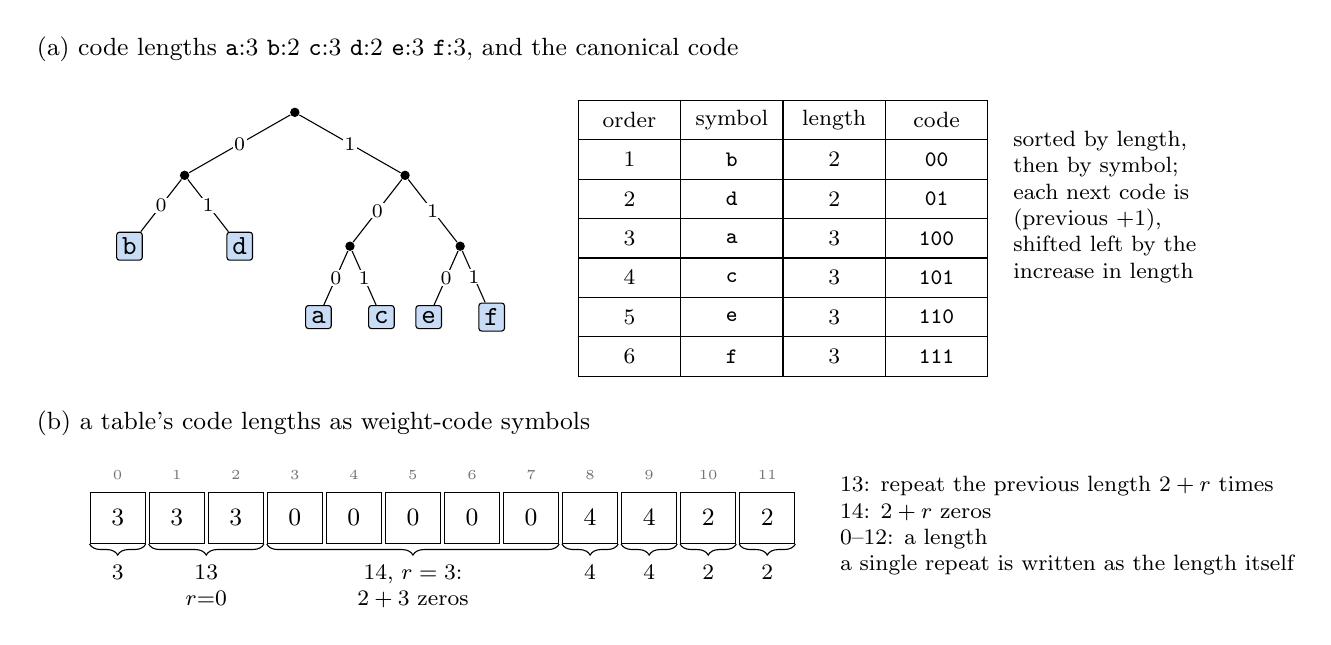
\begin{tikzpicture}[font=\small,
  cell/.style={draw, minimum width=7mm, minimum height=6.5mm, inner sep=0pt},
  dot/.style={circle, fill, inner sep=1.2pt},
  leaf/.style={draw, fill=tok, rounded corners=1pt, inner sep=2pt, font=\ttfamily}]
\node[anchor=west] at (-0.4,1.0) {(a) code lengths \texttt{a}:3 \texttt{b}:2 \texttt{c}:3 \texttt{d}:2 \texttt{e}:3 \texttt{f}:3, and the canonical code};
\node[dot] (r) at (3.0,0.2) {};
\node[dot] (n0) at (1.6,-0.6) {}; \node[dot] (n1) at (4.4,-0.6) {};
\node[leaf] (b) at (0.9,-1.5) {b}; \node[leaf] (d) at (2.3,-1.5) {d};
\node[dot] (n10) at (3.7,-1.5) {}; \node[dot] (n11) at (5.1,-1.5) {};
\node[leaf] (a) at (3.3,-2.4) {a}; \node[leaf] (c) at (4.1,-2.4) {c};
\node[leaf] (e) at (4.7,-2.4) {e}; \node[leaf] (f) at (5.5,-2.4) {f};
\foreach \p/\q/\l in {r/n0/0, r/n1/1, n0/b/0, n0/d/1, n1/n10/0, n1/n11/1, n10/a/0, n10/c/1, n11/e/0, n11/f/1}
  \draw (\p) -- node[font=\scriptsize, fill=white, inner sep=0.5pt] {\l} (\q);
\foreach \o/\s/\l/\c [count=\i from 0] in {order/symbol/length/code, 1/\texttt{b}/2/\texttt{00}, 2/\texttt{d}/2/\texttt{01},
    3/\texttt{a}/3/\texttt{100}, 4/\texttt{c}/3/\texttt{101}, 5/\texttt{e}/3/\texttt{110}, 6/\texttt{f}/3/\texttt{111}}
  \foreach \t [count=\j from 0] in {\o, \s, \l, \c} {
    \draw (6.6+1.3*\j,0.35-0.5*\i) rectangle ++(1.3,-0.5);
    \node[font=\footnotesize] at (7.25+1.3*\j,0.1-0.5*\i) {\t};}
\node[anchor=west, font=\footnotesize, align=left] at (12.0,-1.0) {sorted by length,\\then by symbol;\\each next code is\\(previous $+1$),\\shifted left by the\\increase in length};
\node[anchor=west] at (-0.4,-3.75) {(b) a table's code lengths as weight-code symbols};
\foreach \v [count=\i] in {3,3,3,0,0,0,0,0,4,4,2,2}
  \node[cell] (L\i) at (0.75*\i,-4.95) {\v};
\foreach \i [evaluate=\i as \s using int(\i-1)] in {1,...,12} \node[font=\tiny, black!55] at (0.75*\i,-4.4) {\s};
\newcommand{\ws}[3]{\draw[mbrc] (L#1.south west) -- (L#2.south east) node[midway, below=4pt, font=\footnotesize, align=center] {#3};}
\ws{1}{1}{3} \ws{2}{3}{13\\$r{=}0$} \ws{4}{8}{14, $r=3$:\\$2+3$ zeros} \ws{9}{9}{4} \ws{10}{10}{4} \ws{11}{11}{2} \ws{12}{12}{2}
\node[anchor=west, font=\footnotesize, align=left] at (9.8,-5.05) {13: repeat the previous length $2+r$ times\\14: $2+r$ zeros\\0--12: a length\\a single repeat is written as the length itself};
\end{tikzpicture}

%% 7. wzip-offsets: offset values and symbols, and the offset cache
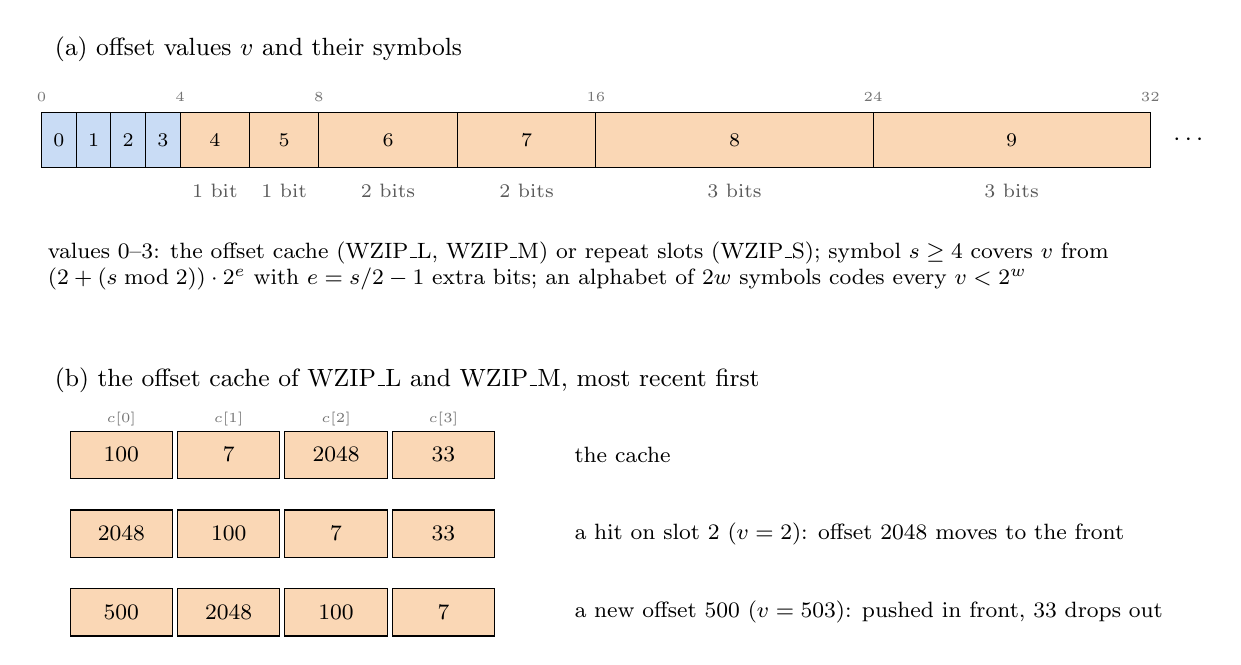
\begin{tikzpicture}[font=\small, x=4.4mm]
\node[anchor=west] at (-0.4,1.15) {(a) offset values $v$ and their symbols};
\newcommand{\rng}[5]{% first value, last value, fill, symbol, extra bits
  \draw[fill=#3] (#1-0.5,-0.35) rectangle (#2+0.5,0.35);
  \node[font=\scriptsize] at ({(#1+#2)/2},0) {#4};
  \node[font=\scriptsize, black!65] at ({(#1+#2)/2},-0.65) {#5};}
\foreach \v in {0,1,2,3} \rng{\v}{\v}{tok}{\v}{};
\rng{4}{5}{off}{4}{1 bit} \rng{6}{7}{off}{5}{1 bit} \rng{8}{11}{off}{6}{2 bits} \rng{12}{15}{off}{7}{2 bits}
\rng{16}{23}{off}{8}{3 bits} \rng{24}{31}{off}{9}{3 bits}
\node at (32.6,0) {$\cdots$};
\foreach \v in {0,4,8,16,24,32} \node[font=\tiny, black!55] at (\v-0.5,0.55) {\v};
\node[font=\footnotesize, align=left, anchor=west] at (-0.6,-1.6) {values 0--3: the offset cache (WZIP\_L, WZIP\_M) or repeat slots (WZIP\_S); symbol $s\ge 4$ covers $v$ from\\$(2+(s\bmod 2))\cdot 2^{e}$ with $e = s/2-1$ extra bits; an alphabet of $2w$ symbols codes every $v<2^w$};
\node[anchor=west] at (-0.4,-3.05) {(b) the offset cache of WZIP\_L and WZIP\_M, most recent first};
\newcommand{\cache}[5]{% y, four entries, note
  \foreach \c [count=\i from 0] in {#2} \node[draw, fill=off, minimum width=13mm, minimum height=6mm, font=\footnotesize] at (1.8+3.1*\i,#1) {\c};
  \node[anchor=west, font=\footnotesize, align=left] at (14.6,#1) {#3};}
\cache{-4.0}{100,7,2048,33}{the cache}{}{}
\cache{-5.0}{2048,100,7,33}{a hit on slot 2 ($v=2$): offset 2048 moves to the front}{}{}
\cache{-6.0}{500,2048,100,7}{a new offset 500 ($v=503$): pushed in front, 33 drops out}{}{}
\foreach \i in {0,1,2,3} \node[font=\tiny, black!55] at (1.8+3.1*\i,-3.55) {$c[\i]$};
\end{tikzpicture}

%% 8. wzip-m: a WZIP_M payload and its two sequence streams
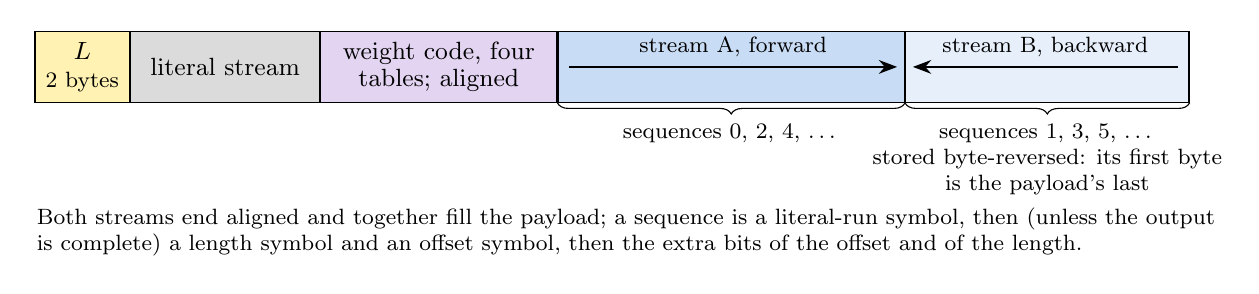
\begin{tikzpicture}[font=\small, node distance=0pt]
\node[fld, fill=hdr, minimum width=12mm, align=center] (l) at (0.6,0) {$L$\\[-1pt]\footnotesize 2 bytes};
\node[fld, fill=lit, minimum width=24mm, right=of l] (ls) {literal stream};
\node[fld, fill=tab, minimum width=30mm, right=of ls, align=center] (tb) {weight code, four\\[-1pt]tables; aligned};
\node[fld, fill=tok, minimum width=44mm, right=of tb] (sa) {};
\node[fld, fill=tok!45, minimum width=36mm, right=of sa] (sb) {};
\draw[-{Stealth}, thick] ($(sa.west)+(0.15,0)$) -- node[above, font=\footnotesize] {stream A, forward} ($(sa.east)+(-0.1,0)$);
\draw[-{Stealth}, thick] ($(sb.east)+(-0.15,0)$) -- node[above, font=\footnotesize] {stream B, backward} ($(sb.west)+(0.1,0)$);
\draw[mbrc] (sa.south west) -- (sa.south east) node[midway, below=4pt, font=\footnotesize] {sequences 0, 2, 4, \ldots};
\draw[mbrc] (sb.south west) -- (sb.south east) node[midway, below=4pt, font=\footnotesize, align=center] {sequences 1, 3, 5, \ldots\\stored byte-reversed: its first byte\\is the payload's last};
\node[anchor=west, font=\footnotesize, align=left] at (-0.1,-2.1) {Both streams end aligned and together fill the payload; a sequence is a literal-run symbol, then (unless the output\\is complete) a length symbol and an offset symbol, then the extra bits of the offset and of the length.};
\end{tikzpicture}

%% 9. wzip-s: a WZIP_S header and a four-stream body
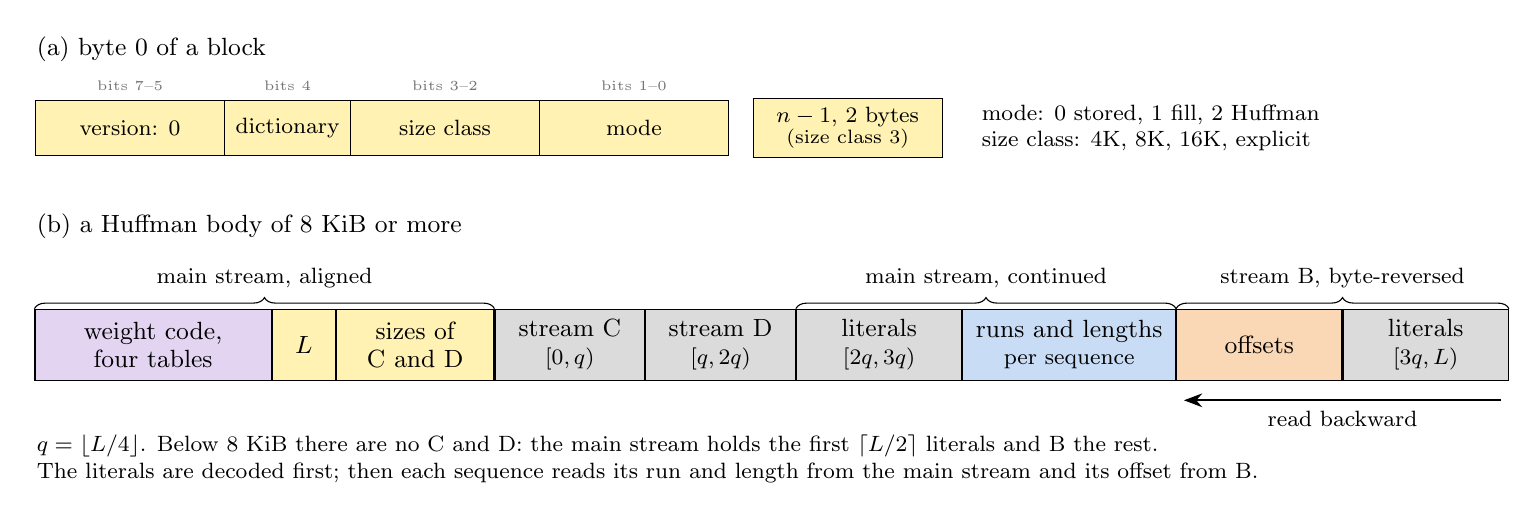
\begin{tikzpicture}[font=\small, node distance=0pt]
\node[anchor=west] at (-0.1,1.0) {(a) byte 0 of a block};
\foreach \b/\w/\t/\x [count=\i from 0] in {{7--5}/24/{version: 0}/0, 4/16/{dictionary}/2.4, {3--2}/24/{size class}/4.0, {1--0}/24/{mode}/6.4} {
  \node[draw, fill=hdr, minimum width=\w mm, minimum height=7mm, anchor=west, font=\footnotesize] (hb\i) at (\x,0) {\t};
  \node[font=\tiny, black!55, above=0pt of hb\i] {bits \b};}
\node[draw, fill=hdr, minimum width=24mm, minimum height=7mm, right=3mm of hb3, font=\footnotesize, align=center] {$n-1$, 2 bytes\\[-2pt]\scriptsize (size class 3)};
\node[anchor=west, font=\footnotesize, align=left] at (11.9,0) {mode: 0 stored, 1 fill, 2 Huffman\\size class: 4K, 8K, 16K, explicit};
\node[anchor=west] at (-0.1,-1.25) {(b) a Huffman body of 8 KiB or more};
\node[fld, fill=tab, minimum width=30mm, align=center] (m1) at (1.5,-2.75) {weight code,\\[-1pt]four tables};
\node[fld, fill=hdr, minimum width=8mm, right=of m1] (m2) {$L$};
\node[fld, fill=hdr, minimum width=20mm, right=of m2, align=center] (m3) {sizes of\\[-1pt]C and D};
\node[fld, fill=lit, minimum width=19mm, right=of m3, align=center] (sc) {stream C\\[-1pt]\footnotesize $[0,q)$};
\node[fld, fill=lit, minimum width=19mm, right=of sc, align=center] (sd) {stream D\\[-1pt]\footnotesize $[q,2q)$};
\node[fld, fill=lit, minimum width=21mm, right=of sd, align=center] (ma) {literals\\[-1pt]\footnotesize $[2q,3q)$};
\node[fld, fill=tok, minimum width=27mm, right=of ma, align=center] (ms) {runs and lengths\\[-1pt]\footnotesize per sequence};
\node[fld, fill=off, minimum width=21mm, right=of ms, align=center] (bo) {offsets};
\node[fld, fill=lit, minimum width=21mm, right=of bo, align=center] (bl) {literals\\[-1pt]\footnotesize $[3q,L)$};
\draw[brc] (m1.north west) -- (m3.north east) node[midway, above=4pt, font=\footnotesize] {main stream, aligned};
\draw[brc] (ma.north west) -- (ms.north east) node[midway, above=4pt, font=\footnotesize] {main stream, continued};
\draw[brc] (bo.north west) -- (bl.north east) node[midway, above=4pt, font=\footnotesize] {stream B, byte-reversed};
\draw[-{Stealth}, thick] ($(bl.south east)+(-0.1,-0.25)$) -- node[below, font=\footnotesize] {read backward} ($(bo.south west)+(0.1,-0.25)$);
\node[anchor=west, font=\footnotesize, align=left] at (-0.1,-4.2) {$q = \lfloor L/4\rfloor$. Below 8 KiB there are no C and D: the main stream holds the first $\lceil L/2\rceil$ literals and B the rest.\\The literals are decoded first; then each sequence reads its run and length from the main stream and its offset from B.};
\end{tikzpicture}

%% 10. wzip-size: the size field, and what a decoder derives from it
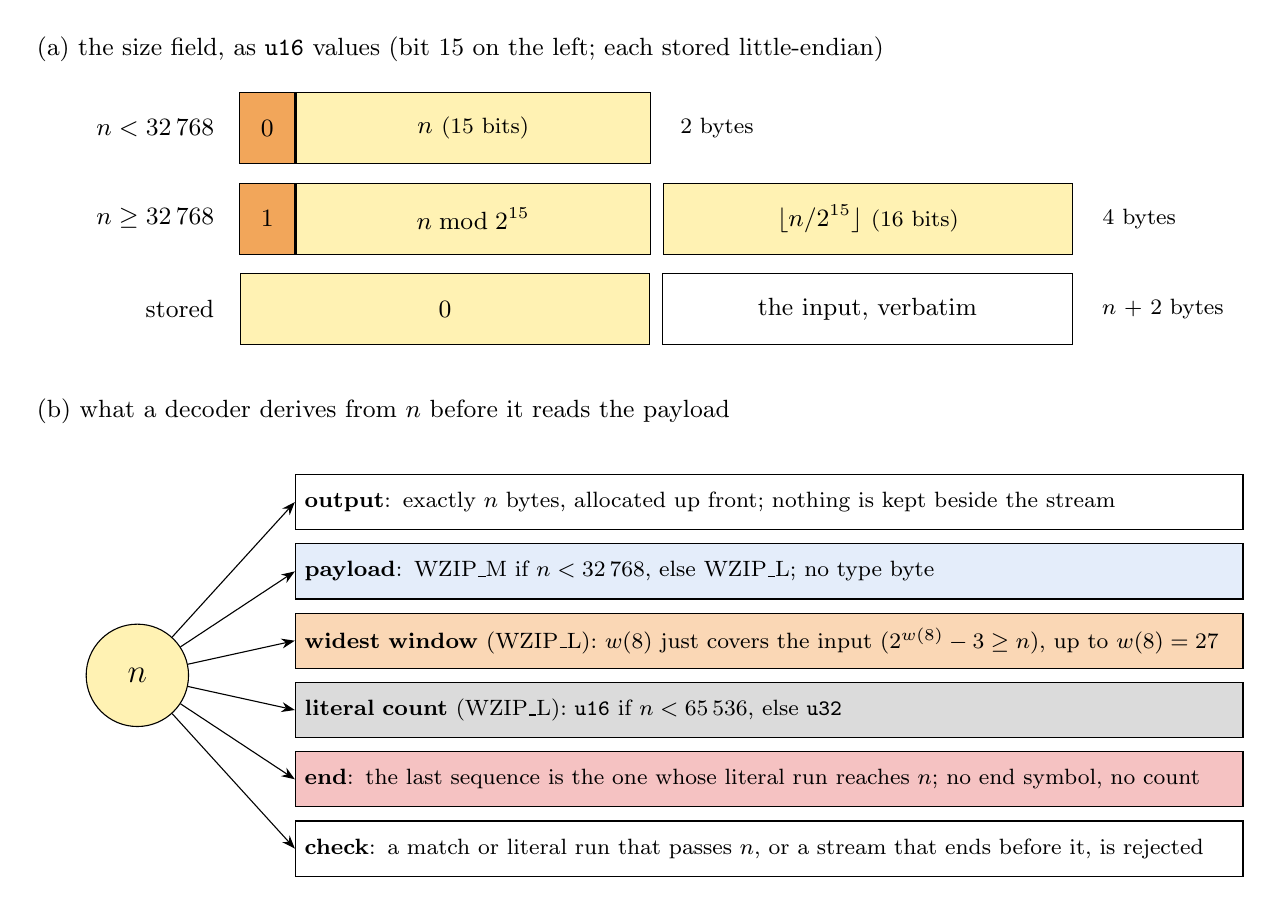
\begin{tikzpicture}[font=\small, node distance=0pt]
\node[anchor=west] at (-0.1,1.0) {(a) the size field, as \texttt{u16} values (bit 15 on the left; each stored little-endian)};
\node[anchor=east] at (2.4,0) {$n<32\,768$};
\node[fld, fill=flg, minimum width=7mm] (f1) at (2.95,0) {0};
\node[fld, fill=hdr, minimum width=45mm, right=of f1] (v1) {$n$ \footnotesize (15 bits)};
\node[anchor=west, font=\footnotesize] at ($(v1.east)+(0.25,0)$) {2 bytes};
\node[anchor=east] at (2.4,-1.15) {$n\ge 32\,768$};
\node[fld, fill=flg, minimum width=7mm] (f2) at (2.95,-1.15) {1};
\node[fld, fill=hdr, minimum width=45mm, right=of f2] (v2) {$n \bmod 2^{15}$};
\node[fld, fill=hdr, minimum width=52mm, right=1.5mm of v2] (v3) {$\lfloor n / 2^{15}\rfloor$ \footnotesize (16 bits)};
\node[anchor=west, font=\footnotesize] at ($(v3.east)+(0.25,0)$) {4 bytes};
\node[anchor=east] at (2.4,-2.3) {stored};
\node[fld, fill=hdr, minimum width=52mm, anchor=west] (s1) at (2.6,-2.3) {0};
\node[fld, minimum width=52mm, right=1.5mm of s1] (s2) {the input, verbatim};
\node[anchor=west, font=\footnotesize] at ($(s2.east)+(0.25,0)$) {$n$ + 2 bytes};
\node[anchor=west] at (-0.1,-3.6) {(b) what a decoder derives from $n$ before it reads the payload};
\node[draw, circle, fill=hdr, minimum size=13mm, font=\large] (n) at (1.3,-6.95) {$n$};
\foreach \f/\t [count=\i from 0] in {
    white/{\textbf{output}: exactly $n$ bytes, allocated up front; nothing is kept beside the stream},
    tok!50/{\textbf{payload}: WZIP\_M if $n<32\,768$, else WZIP\_L; no type byte},
    off/{\textbf{widest window} (WZIP\_L): $w(8)$ just covers the input ($2^{w(8)}-3\ge n$), up to $w(8)=27$},
    lit/{\textbf{literal count} (WZIP\_L): \texttt{u16} if $n<65\,536$, else \texttt{u32}},
    endm/{\textbf{end}: the last sequence is the one whose literal run reaches $n$; no end symbol, no count},
    white/{\textbf{check}: a match or literal run that passes $n$, or a stream that ends before it, is rejected}} {
  \node[draw, fill=\f, anchor=west, minimum height=7mm, text width=118mm, align=left, font=\footnotesize]
    (d\i) at (3.3,-4.75-0.88*\i) {\t};
  \draw[-{Stealth}] (n) -- (d\i.west);}
\end{tikzpicture}

\end{document}
